
\chapter{Multi-Objective Optimization}
\todoChapter{ 10\% complete. Goal 80\% completion date: July 20\\
Notes: Clean up this section.  Add more information.}

\begin{outcome}
\begin{itemize}
\item Define multi objective optimization problems
\item Discuss the solutions in terms of the \emph{Pareto Frontier}
\item Explore approaches for finding the Pareto Frontier
\item Use software to solve for or approximate the Pareto Frontier
\end{itemize}
\end{outcome}

\begin{resource}
\href{https://pymoo.org/}{Python Multi Objective Optimization (Pymoo)}
\end{resource}

\section{Multi Objective Optimization and The Pareto Frontier}
On Dealing with Ties and Multiple Objectives in Linear Programming



Consider a high end furniture manufacturer which builds dining tables and chairs out of expensive bocote and rosewood.

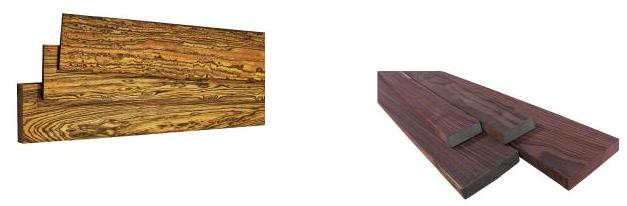
\includegraphics[width=0.5\textwidth]{optimization/multi-objective/images/2022_02_28_634e8079070800ac7e3cg-02}

The manufacturer has an ongoing deal with a foreign sawmill which supplies them with 960 and 200 board-feet (bdft) of bocote and rosewood respectively each month.

A single table requires 80 bdft of bocote and 20 bdft of rosewood.

Each chair requires only 20 bdft of bocote but 10 bdft of rosewood.
$$
\begin{aligned}
P=\{&(x, y) \in \mathbb{R}^{2}: \\
& 80 x+20 y \leq 960 \\
& 12 x+10 y \leq 200 \\
&x, y \geq 0\}
\end{aligned}
$$
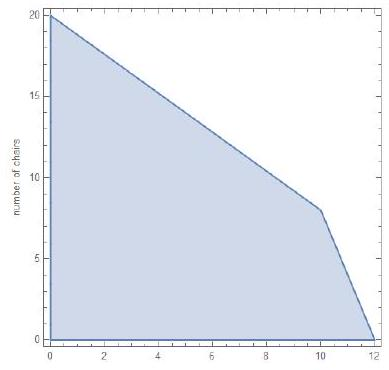
\includegraphics[width=0.5\textwidth]{optimization/multi-objective/images/2022_02_28_634e8079070800ac7e3cg-03}

Suppose that each table will sells for $\$ 7000$ while a chair goes for $\$ 1500 .$ To increase profit we want to maximize
$$
F(x, y)=8000 x+2000 y
$$
over $P$. Having taken a linear programming class, the manager knows his way around these problems and begins the simplex method:

Maximize $8000 x+2000 y$

s.t. $\quad 80 x+20 y \leq 960$
$$
12 x+10 y \leq 200
$$
$$
\begin{aligned}
& x, y \geq 0
\end{aligned}
$$
\begin{tabular}{llll|l}
$-4$ & $-1$ & 0 & 0 & 0 \\
\hline
4 & 1 & 1 & 0 & 48 \\
6 & 5 & 0 & 1 & 100 \\
\end{tabular}

Maximize $4 x+y$

s.t. $\quad 4 x+y+s_{1}=48$
$$
\begin{aligned}
& \begin{aligned}\frac{f}{2000} & \begin{aligned}6 x+5 y+s_{2} &=100 \\x, y & \geq 0\end{aligned}\end{aligned} 
\end{aligned}
$$
Having found an optimal solution, the manager is quick to set up production. The best thing to do is produce 12 tables a month and no chairs!

But there are actually multiple optima!

How could we have noticed this this from the tableau? From the original formulation?

Is the manager's solution really the best?

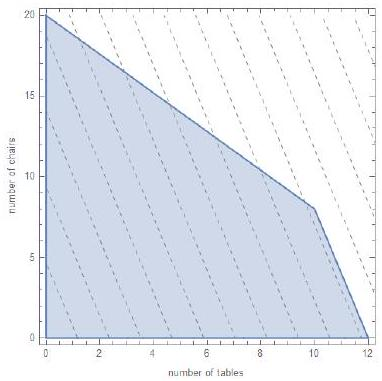
\includegraphics[width=0.5\textwidth]{optimization/multi-objective/images/2022_02_28_634e8079070800ac7e3cg-05}

number of tables Having fired the prior manager for producing no chairs, a new and more competent manager is hired. This one knows that Dalbergia stevensonii (the tree which produces their preferred rosewood) is a threatened species and decides that she doesn't want to waste any more rosewood than is necessary.

After some investigation, she finds that table production wastes nearly 10 bdft of rosewood per table while chairs are dramatically more efficient wasting only 2 bdft per chair. She comes up with a new, secondary objective function that she would like to minimize:
$$
w(x, y)=10 x+2 y .
$$
Having noticed that there are multiple profit-maximizers, she formulates a new problem to break the tie:
$$
\begin{aligned}
\text { Minimize } 10 x+2 y & \\
\text { s.t. } \quad 80 x+20 y &=960 \\
x & \in[10,12] \\
y & \in[0,8] .
\end{aligned}
$$
This is easy in this case because the set of profit-optimal solutions is simple.

Because this is an LP, the optimal solution will be at an extreme point; there are only two here, so the problem reduces to
$$
\arg \min \{10 x+2 y:(x, y) \in\{(12,0),(10,8)\}\}
$$
Therefore, swapping out some tables for chairs reduces waste and without affecting revenue!

What the manager just did is called the Ordered Criteria or Lexicographic method for Multi-Objective Optimization. After a few months, the manager convinces the owners that reducing waste is worth a small loss in profit. The owners concede to a $30 \%$ loss in revenue and our manager gets to work on a new model:
$$
\begin{aligned}
\text { Minimize } & 10 x+2 y \\
\text { s.t. } \quad 8000 x+2000 y & \geq(\alpha) 96000 \\
80 x+20 y & \leq 960 \\
12 x+10 y & \leq 200 \\
x, y & \geq 0
\end{aligned}
$$
where $\alpha=0.7$ This new constraint limits us to solutions which offered at least $70 \%$ of maximum possible revenue.

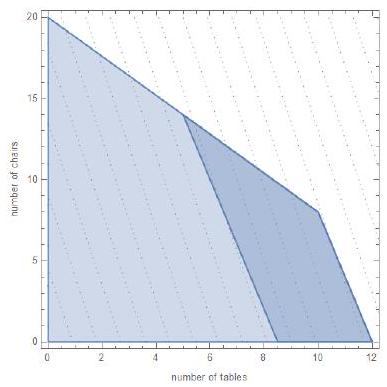
\includegraphics[width=0.5\textwidth]{optimization/multi-objective/images/2022_02_28_634e8079070800ac7e3cg-10}

The strategy is the called the Benchmark or Rollover method because we choose a benchmark for one of our objectives (revenue in this case), roll that benchmark into the constraints, and optimize for the second objective (waste).

Notice that if we set $\alpha$ to 1 , the rollover problem is equivalent to the lexicographic problem. Either approach requires a known optimal value to the first objective function.

Interestingly, our rollover solution is NOT an extreme point to the ORIGINAL feasible region. Given a set $P$ and some number of functions $f_{i}: P \rightarrow \mathbb{R}$ that we seek to maximize, we call a point $\mathbf{x} \in P$ Pareto Optimal or Efficient if there does not exist another point $\overline{\mathbf{x}} \in P$ such that

\begin{itemize}
  \item $f_{i}(\overline{\mathbf{x}})>f_{i}(\mathbf{x})$ for some $i$ and
\end{itemize}
$\rightarrow f_{j}(\overline{\mathbf{x}}) \geq f_{j}(\mathbf{x})$ for all $j \neq i$.

That is, we cannot make any objective better without making some other objective worse.

The Pareto Frontier is the set of all Pareto optimal points for some problem. Which of these points is Pareto optimal?

What is the frontier of this problem?

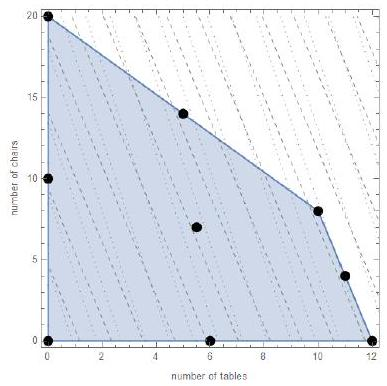
\includegraphics[width=0.5\textwidth]{optimization/multi-objective/images/2022_02_28_634e8079070800ac7e3cg-13}

number of tables The rollover method is generalized in Goal Programming

By varying $\alpha$, it is possible to generate many distinct efficient solutions.

However, this method can generate inefficient solutions if the underlying model is poorly constructed.

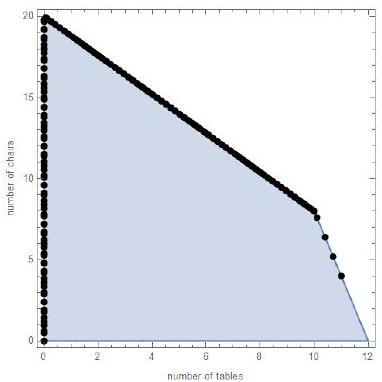
\includegraphics[width=0.5\textwidth]{optimization/multi-objective/images/2022_02_28_634e8079070800ac7e3cg-14}

number of tables It is more common to see a Pareto frontier plotted with respect to its objectives.

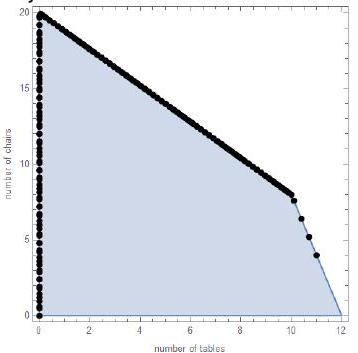
\includegraphics[width=0.5\textwidth]{optimization/multi-objective/images/2022_02_28_634e8079070800ac7e3cg-15}

number of table

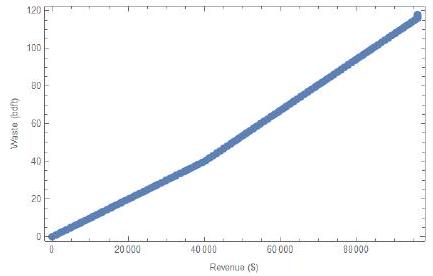
\includegraphics[width=0.5\textwidth]{optimization/multi-objective/images/2022_02_28_634e8079070800ac7e3cg-15(1)}

One of the owners of our manufactory decides to explore possible planning himself; he implements the multi-objective method that he remembers, Scalarization by picking some arbitrary constant $\lambda \in[0,1]$ and combining his two objectives like so:
$$
\begin{array}{cl}
\text { Minimize } & \lambda(8000 x+2000 y)+(1-\lambda)(10 x+2 y) \\
\text { s.t. } & 80 x+20 y \leq 960 \\
& 12 x+10 y \leq 200 \\
& x, y \geq 0
\end{array}
$$
What is the benefit of this method?

Where does it fall short?

\section{What points will the Scalarization method find if we vary $\lambda ?$}
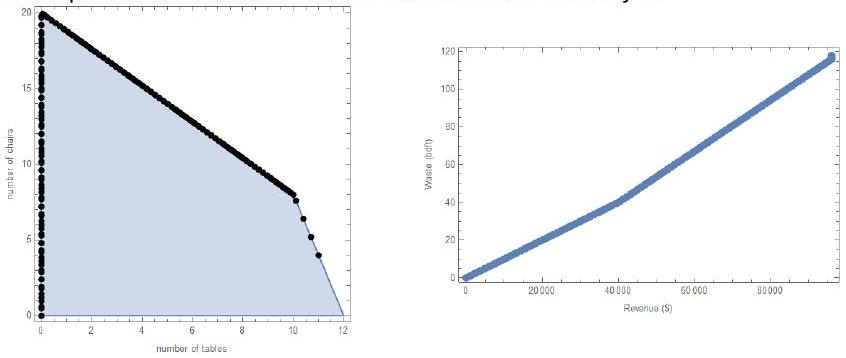
\includegraphics[width=0.5\textwidth]{optimization/multi-objective/images/2022_02_28_634e8079070800ac7e3cg-17}These are all nice ideas, but the problem presented above is neither difficult nor practical.

What are some areas that a Pareto frontier would be actually useful?

\section{Political Redistricting [3]}
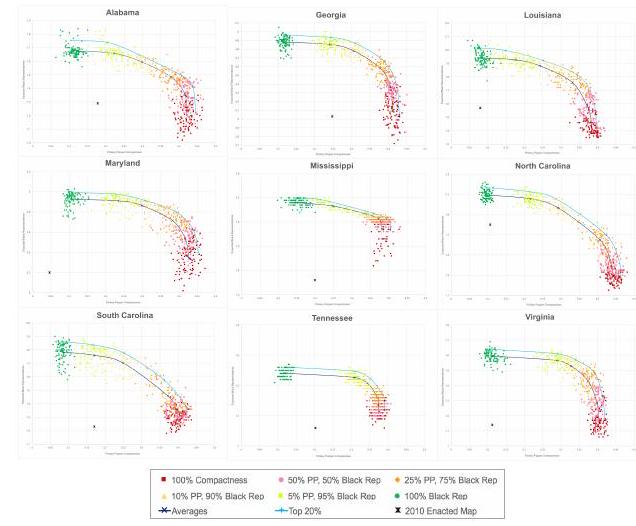
\includegraphics[width=0.5\textwidth]{optimization/multi-objective/images/2022_02_28_634e8079070800ac7e3cg-19}

\section{Portfolio Optimization [5]}
\section{Simulated Portfolio Optimization based on Efficient Frontier}
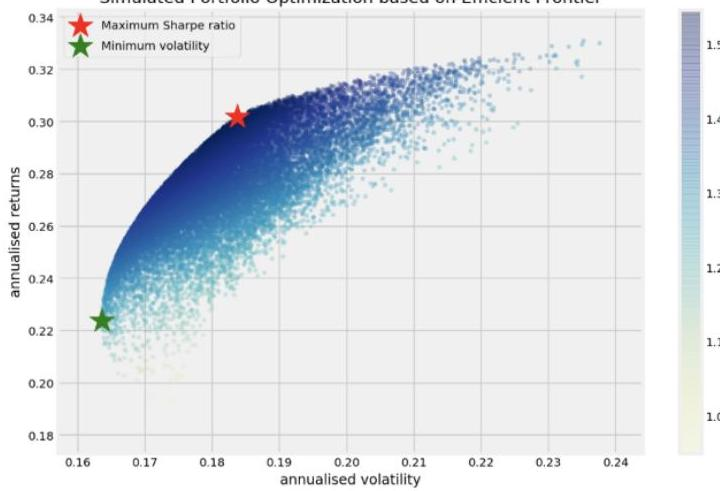
\includegraphics[width=0.5\textwidth]{optimization/multi-objective/images/2022_02_28_634e8079070800ac7e3cg-20}

\section{Aircraft Design [1]}
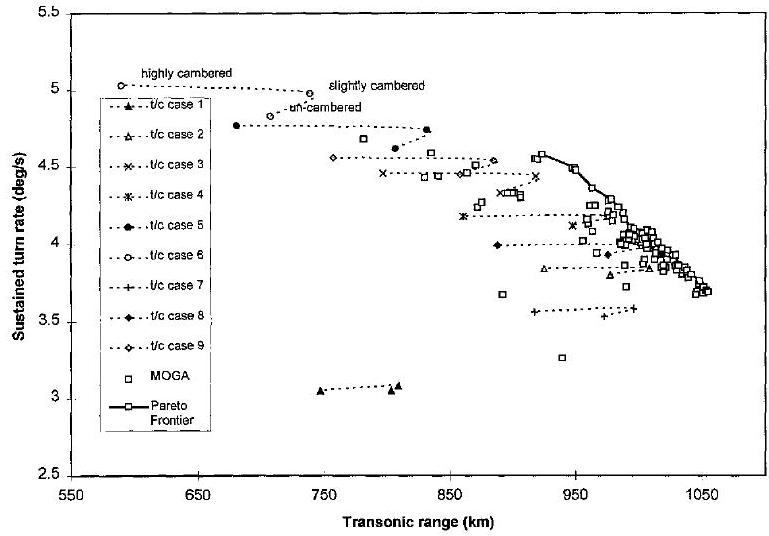
\includegraphics[width=0.5\textwidth]{optimization/multi-objective/images/2022_02_28_634e8079070800ac7e3cg-21}

\section{Vehicle Dynamics [4]}
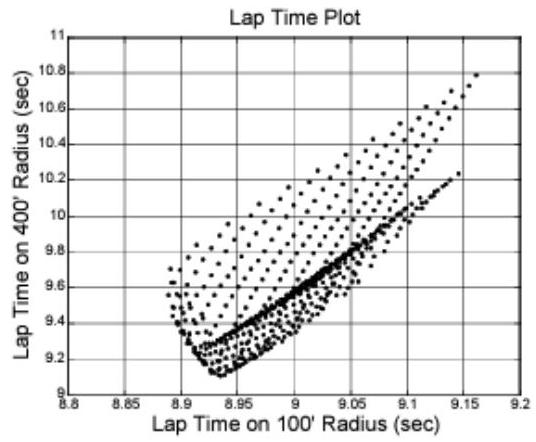
\includegraphics[width=0.5\textwidth]{optimization/multi-objective/images/2022_02_28_634e8079070800ac7e3cg-22}

Figure 7: Grid Search Results in the Performance Space

\section{Sustainable Constriction [2]}
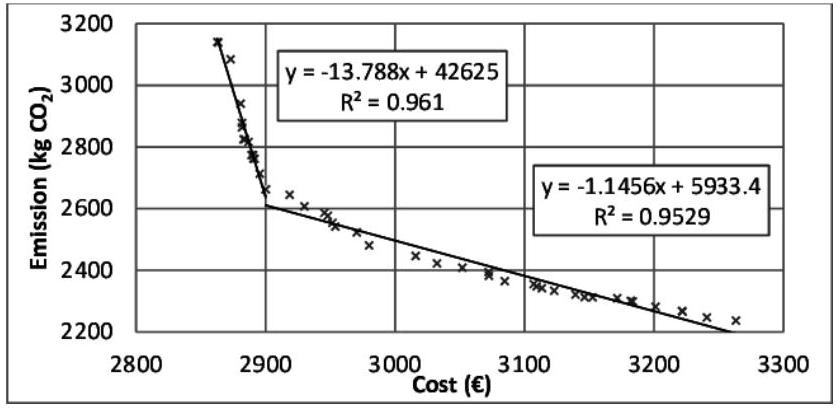
\includegraphics[width=0.5\textwidth]{optimization/multi-objective/images/2022_02_28_634e8079070800ac7e3cg-23}

\section{References}
S. Fenwick and John C. Harris. the application of pareto frontier methods in the multidisciplinary wing design of a generic modern military delta aircraft: Semantic scholar, Jan $1999 .$

URL: \href{https://WWW}{https://WWW}. semanticscholar. org/paper/

The-application-of-Pareto-frontier-methods-in-the-a-Fenwick-Harris/ fced $00 a 59 \mathrm{~d} 200 c 2 c 74$ ed 655 a 457344 bcleea 6 ff $5 .$

T García-Segura, V Yepes, and J Alcalá.

Sustainable design using multiobjective optimization of high-strength concrete i-beams. In The 2014 International Conference on High Performance and Optimum Design of Structures and Materials HPSM/OPTI, volume 137, pages $347-358,2014 .$

URL: \href{https://www}{https://www}. \href{http://researchgate.net/publication/271439836_Sustainable_design_using_}{researchgate.net/publication/271439836\_Sustainable\_design\_using\_} multiobjective\_optimization\_of\_high-strength\_concrete\_l-beams.

Nicholas Goedert, Robert Hildebrand, Laurel Travis, Matthew Pierson, and Jamie Fravel. Black representation and district compactness in southern congressional districts. not yet published, ask Dr. Hildebrand for it.

Edward M Kasprzak and Kemper E Lewis.

Pareto analysis in multiobjective optimization using the collinearity theorem and scaling method. Structural and Multidisciplinary Optimization.

Ricky Kim.

Efficient frontier portfolio optimisation in python, Jun $2021 .$

URL: \href{https://towardsdatascience}{https://towardsdatascience}. com/

efficient-frontier-portfolio-optimisation-in-python-e7844051e7f.


%\end{document}